\chapter{Segmentation, step by step}
\label{chap:segmentation}

This chapter follows the pipeline of Figure~\ref{fig:pipeline}. For each step: what the image
looks like, what the step does, and what it changed. I produced the ``before'' images by checking
out the corresponding past version of the code and running it on the same data
(Appendix~\ref{chap:reproduce}).

\section{One set of thresholds for the whole stack}
\label{sec:thresholds}

The three materials are visible as three modes of the intensity histogram
(Figure~\ref{fig:histogram}). A 3-class Otsu threshold maximises the between-class variance over every
pair of thresholds. pyBones runs it once, on the histogram of every fifth slice (after a light
Gaussian denoising), with an exhaustive search vectorised over a $1024 \times 1024$ grid of threshold
pairs. When the optimum is a plateau (an empty gap in the histogram), the centre of the plateau is
taken rather than its first element, which would sit on the tail of a class.

\begin{figure}[ht]
\centering
\begin{tikzpicture}
\begin{axis}[width=0.9\linewidth,height=5.2cm,ymode=log,xmin=0,xmax=45000,
  xlabel={intensity (16-bit grey level)},ylabel={fraction of voxels},
  tick label style={font=\small},label style={font=\small},
  scaled x ticks=false,xticklabel style={/pgf/number format/1000 sep={\,}}]
  \addplot[ink,thick] table[x=intensity,y=fraction,col sep=comma]{data/histogram.csv};
  \draw[accent,dashed,thick] (axis cs:\pbNumThrBone,1e-7) -- (axis cs:\pbNumThrBone,1);
  \draw[accent,dashed,thick] (axis cs:\pbNumThrVessel,1e-7) -- (axis cs:\pbNumThrVessel,1);
  \node[font=\footnotesize,anchor=south] at (axis cs:\pbNumMeanBackground,2e-2) {soft tissue};
  \node[font=\footnotesize,anchor=south,boneC!70!black] at (axis cs:\pbNumMeanBone,4e-3) {bone};
  \node[font=\footnotesize,anchor=south,vesselC] at (axis cs:\pbNumMeanVessel,1e-4) {contrast agent};
\end{axis}
\end{tikzpicture}
\caption{Histogram of the (smoothed) stack, log scale, with the two global thresholds
  (\pbValueThrBone{} and \pbValueThrVessel). The class means are \pbValueMeanBackground,
  \pbValueMeanBone{} and \pbValueMeanVessel.}
\label{fig:histogram}
\end{figure}

Per-slice thresholds, as in 2018, barely varied on this stack, but a single set guarantees that the
same tissue gets the same class everywhere, which every later 3D step relies on.

\section{Vessel edges at half-maximum}
\label{sec:edges}

\paragraph{The physics} A scanner blurs the image: every voxel averages the materials around it. A
voxel half filled with contrast agent and half with soft tissue reads halfway between the two
intensities; a voxel a quarter filled reads a quarter of the way. The natural boundary of a vessel is
therefore the \emph{half-maximum}: the voxels at least half filled with contrast agent. I measured the
blur of this scanner on the bone edges (the maximum gradient of a blurred step of contrast $C$
is $C / (\sigma\sqrt{2\pi})$): $\sigma \approx 1.45$ pixel, about 4.4\um.

\paragraph{The flaw it fixed} My first versions grew vessels from their bright cores down to a fixed
``weak'' threshold that sat at bone level. On the phantom (Chapter~\ref{chap:validation}) vessels came
out 1.75 times too thick, and a vessel lying against bone ate into it. Figure~\ref{fig:profile} shows
the effect on a real vessel: the 2018 mask and the 0.2 mask both extend well past the half-maximum.

\paragraph{The rule} For each candidate pixel near a bright core:
\[
  I \;\ge\; S + f\,(C - S),
\]
where $C$ is the brightest core within the rim radius (a grey-level dilation: the intensity of a fully
filled voxel of \emph{that} vessel, whatever its filling), $S$ the surrounding material, and
$f = 0.5$ the occupancy. The surround is read from the darkest intensity just beyond the rim (a
grey-level erosion): below the bone threshold it is soft tissue and the soft-tissue mean is used,
otherwise it is bone. A vessel running along bone is thus measured against bone and cannot eat into it.

Pixels near a core but below the half-maximum, with soft tissue around, form the \emph{halo}: a
vessel/soft-tissue mix whose intensity can reach bone level. They are background, not bone. This
replaced our 2018 rule, which turned every small blob holding a bright core into a vessel, halo
included.

\paragraph{In 3D} Cores and surround are searched in a 3D ball, not a disk. A vessel lying in the
slice plane blurs into the slices above and below; in those slices there is no bright core within
reach in 2D, so its blur used to become a ``bone collar'' around the vessel
(Figure~\ref{fig:collar}).

\begin{figure}[ht]
\centering
\begin{tikzpicture}
\begin{axis}[width=0.9\linewidth,height=5.6cm,xlabel={position across the vessel ($\mu$m)},
  ylabel={intensity},xmin=0,xmax=177,ymin=0,
  legend style={font=\footnotesize,at={(0.99,0.97)},anchor=north east,draw=none,fill=white,fill opacity=0.8},
  tick label style={font=\small},label style={font=\small},
  yticklabel style={/pgf/number format/1000 sep={\,}},scaled y ticks=false]
  \addplot[legacyC,only marks,mark size=1pt] table[x=x_um,y=raw,col sep=comma]{data/profile.csv};
  \addlegendentry{raw}
  \addplot[ink,thick] table[x=x_um,y=smoothed,col sep=comma]{data/profile.csv};
  \addlegendentry{smoothed}
  \draw[accent,dashed,thick] (axis cs:0,\pbNumProfileHalfMax) -- (axis cs:177,\pbNumProfileHalfMax);
  \node[accent,font=\footnotesize,anchor=south west] at (axis cs:2,\pbNumProfileHalfMax) {half-maximum};
  \addplot[legacyC,line width=4pt,unbounded coords=jump]
    table[x=x_um,y expr={\thisrow{legacy_vessel} > 0 ? 6000 : nan},col sep=comma]{data/profile.csv};
  \addlegendentry{2018 vessel mask}
  \addplot[vesselC!50,line width=4pt,unbounded coords=jump]
    table[x=x_um,y expr={\thisrow{v02_vessel} > 0 ? 3500 : nan},col sep=comma]{data/profile.csv};
  \addlegendentry{0.2 vessel mask}
  \addplot[vesselC,line width=4pt,unbounded coords=jump]
    table[x=x_um,y expr={\thisrow{current_vessel} > 0 ? 1000 : nan},col sep=comma]{data/profile.csv};
  \addlegendentry{\pbValueVersion{} vessel mask}
\end{axis}
\end{tikzpicture}
\caption{Intensity across a bright vessel (slice 0), and the extent of the vessel mask of each version
  (bars at the bottom). The half-maximum between the soft tissue and this vessel's core
  (\pbValueProfileCore) is \pbValueProfileHalfMax.}
\label{fig:profile}
\end{figure}

\begin{figure}[p]
\centering
\panel{0.24}{edges_vessels_raw.jpg}{Raw.}\hfill
\panel{0.24}{edges_vessels_v02.jpg}{0.2: fixed threshold.}\hfill
\panel{0.24}{edges_vessels_halfmax.jpg}{Half-maximum (2D).}\hfill
\panel{0.24}{edges_vessels_current.jpg}{\pbValueVersion: half-maximum in 3D.}
\caption{Marrow vessels. The fixed threshold of 0.2 draws the vessels wider than they appear; the
  half-maximum draws them at their visible width.}
\label{fig:edges}
\bigskip
\panel{0.24}{collar_raw.jpg}{Raw.}\hfill
\panel{0.24}{collar_halfmax.jpg}{Half-maximum (2D).}\hfill
\panel{0.24}{collar_tubes.jpg}{With the plate veto.}\hfill
\panel{0.24}{collar_current.jpg}{\pbValueVersion: 3D halo.}
\caption{A vessel lying in the slice plane, in soft tissue (lower vessel). Its blur in the neighbouring
  slices has no core within reach in 2D: first a vessel sheath, then (once plate-like blobs could not be
  vessels) a bone collar. Searching the cores in 3D removes most of it; a thin remnant remains on one
  side.}
\label{fig:collar}
\end{figure}

\section{Bursts}
\label{sec:bursts}

A burst is a cloud of contrast agent: a dense cluster of bright speckles, a few hundred micrometres
across (230 to 450\um{} on this scan). A thin vessel, even a bright one, is sparse at that scale.
I therefore measure the \emph{density} of bright pixels in a 123\um{} box around each pixel
(a box filter: integral-image speed), and declares a burst core where it exceeds 35\,\%.

\paragraph{In 3D} Measured per slice, the density flickers: near the top and bottom of a cluster a
slice only shows a sparse cross-section. Summing the per-slice densities over 41 slices (a running sum,
one addition and one subtraction per slice) gives the density in a 3D box, consistent along $z$. A cube
alone, however, erodes the ends of a cluster by up to half its depth: during development it lost a
whole cluster at slice 55. The final core is the union of the slice's own 2D core and the 3D core,
the latter only where the slice actually contains contrast agent (so a dense cluster cannot paint the
slices past its end). The density is stored on a 12\um{} grid, sixteen times smaller than per pixel,
since it is a mean over a much larger box.

\paragraph{The boundary} Our 2018 code and my early versions closed the core with a 45\um{} disk and
added an 18\um{} halo. On the phantom, I found every burst error 2 to 16 pixels on either side of the true
boundary: the radii imposed it. The boundary is now placed like the vessel edges, at a half-maximum: the
core grows over the pixels whose fine-scale density (36\um) stays above half the core density, then the
enclosed holes are filled (a purely topological operation, no radius).

\begin{figure}[ht]
\centering
\panel{0.24}{bursts_raw.jpg}{Raw (slice 55).}\hfill
\panel{0.24}{bursts_v02.jpg}{0.2: 2D density.}\hfill
\panel{0.24}{bursts_bursts3d.jpg}{3D density.}\hfill
\panel{0.24}{bursts_current.jpg}{\pbValueVersion: half-density edge.}
\caption{A burst cluster. Bursts are blue, vessels red.}
\label{fig:bursts}
\end{figure}

\begin{figure}[ht]
\centering
\begin{tikzpicture}
\begin{axis}[width=0.9\linewidth,height=5cm,xlabel={slice},ylabel={burst area (\% of the slice)},
  xmin=0,xmax=99,legend style={font=\footnotesize,at={(0.99,0.97)},anchor=north east,draw=none},
  tick label style={font=\small},label style={font=\small}]
  \addplot[legacyC,thick] table[x=z,y expr=100*\thisrow{v02},col sep=comma]{data/bursts_by_slice.csv};
  \addlegendentry{0.2 (2D density)}
  \addplot[burstC!60,thick] table[x=z,y expr=100*\thisrow{bursts3d},col sep=comma]{data/bursts_by_slice.csv};
  \addlegendentry{3D density}
  \addplot[burstC!80!black,thick] table[x=z,y expr=100*\thisrow{current},col sep=comma]{data/bursts_by_slice.csv};
  \addlegendentry{\pbValueVersion}
\end{axis}
\end{tikzpicture}
\caption{Burst area per slice on the real stack. A 3D object should change smoothly from one slice to
  the next; the 2D density makes it jump.}
\label{fig:bursts-z}
\end{figure}

\section{Ambiguous blobs and 3D connectivity}
\label{sec:refinement}

After the vessel edges and the bursts, the remaining bone-intensity regions are split by size: large
connected regions are bone, small ones (under 6300\umsq{} in the slice) are \emph{ambiguous}. A small
blob can be the cross-section of a trabecular rod, or a dim, clotted vessel: these are the ``zones of
uncertainty'' the researchers pointed out to us in 2018. In 3D the question has an answer: a rod joins the bone network, a
vessel joins vessels.

\paragraph{3D components without a 3D label volume} A 32-bit label volume of the stack would weigh
1.4\,GB. Instead, each slice is labelled in 2D (OpenCV), its labels are offset into a global numbering,
and labels of consecutive slices that touch (26-neighbourhood) are recorded as graph edges, looking only
at the previous slice. Since distinct 8-connected components of a slice never touch, the diagonal links
only need to be checked on the thin band where the voxel straight below is background; this cut the
time of the whole refinement by almost three in my measurements. The graph is solved once by a vectorised union-find (every root hooks onto its
smallest neighbouring root, then pointer jumping flattens the forest, until no edge spans two trees).
Any slice can later be re-labelled and mapped through the result, so at most two label slices are ever
in memory.

\paragraph{The decision} Each ambiguous 3D component is decided in three streamed passes:
\begin{itemize}
  \item small and isolated: noise, background;
  \item plate-like (Section~\ref{sec:tubularity}): never a vessel; bone if it touches bone,
        background otherwise (the sheath of a vessel, a fascia);
  \item otherwise \vessel{} if it touches vessels more than bone, or if it is isolated (bone cannot
        float), \bone{} if it touches bone.
\end{itemize}
Finally, vessel and bone 3D components smaller than a minimum volume are removed. I kept our 2018
three-slice majority vote available but disabled it: once 3D connectivity exists, it only fragmented the
bone network (783 bone components instead of 45) for no gain.

\section{Tubes versus plates}
\label{sec:tubularity}

The curvature of the intensity tells shapes apart. At each voxel, the Hessian matrix (second
derivatives) has three eigenvalues $|\lambda_1| \le |\lambda_2| \le |\lambda_3|$: a bright tube curves
strongly in two directions ($\lambda_2 \approx \lambda_3 \ll 0$, $\lambda_1 \approx 0$), a bright plate in
one ($\lambda_3 \ll 0$, $\lambda_1 \approx \lambda_2 \approx 0$), a blob in three. The ratio
$R_A = |\lambda_2| / |\lambda_3|$ is close to 1 for a tube and to 0 for a plate, whatever the contrast.

The Hessian is computed at three scales (3, 4.5 and 6\um) from Gaussian derivatives, streamed through
a window of 13 slices: the raw slices are first combined along $z$ with the three derivative kernels,
then filtered in-plane, never storing a volume. The eigenvalues of millions of $3 \times 3$ symmetric
matrices are computed in closed form (Smith's trigonometric formula), in chunks, only on the voxels that
can become ambiguous.

\paragraph{What it can and cannot do} I tried Frangi's classic vesselness filter first. On the phantom
it separated vessels from bone pieces only through contrast; on shape alone it did no better than
chance: trabecular rods \emph{are} tubes. Plates, however, are separated very well: the mean $R_A$ of
an ambiguous component distinguished true vessels from bone pieces with an area under the ROC curve of
0.93. I therefore use $R_A$ for one thing only, a veto: a component whose mean ratio is below
0.45 cannot be a vessel (Figure~\ref{fig:tubularity}). On the phantom it corrected the largest
misclassified bone fragments (two of them 6\,000 and 17\,000 voxels) without losing any true vessel.

\begin{figure}[ht]
\centering
\panel{0.4}{tubularity_raw.jpg}{Raw (slice 50, marrow).}\hspace{0.05\linewidth}
\panel{0.4}{tubularity_map.jpg}{Mean tube-vs-plate ratio per blob.}
\caption{Ambiguous blobs coloured by their mean ratio $R_A$: blue blobs are plate-like (vetoed),
  green to red ones tube-like. The 3D decision uses the mean over each 3D component; this is its 2D view.}
\label{fig:tubularity}
\end{figure}

\section{Meshing}
\label{sec:meshing}

Surfaces are extracted per label with marching cubes (scikit-image, the only use of that library).
The label volume is first downsampled by an exact block mean, which keeps sub-voxel information and
divides the memory by $8$ (factor 2). Marching cubes on voxel data produces ``staircase'' surfaces
(the ``cubic aspect'' noted in 2018): on a voxelised sphere the surface area is 8.5\,\% too large.
Taubin's $\lambda|\mu$ smoothing alternates a shrinking and an inflating step, which removes the
staircase without shrinking the object: the area error falls to 0.8\,\% in 10 iterations, the volume
is kept, and a two-voxel-thin tube keeps 92\,\% of its volume (blurring the volume before meshing would
erase it).

Meshes are written in micrometres, in one of two formats. Binary STL, for other software, stores every
triangle with its own three corners as 32-bit floats. Binary glTF (GLB), for the browser, stores each
point once and the triangles as indices into them, and can store the positions as 16-bit integers over
the mesh's bounding box (the \code{KHR\_mesh\_quantization} extension), with 8-bit normals. A point is
then off by at most half of the box size divided by 65\,535 on each axis: 0.05\um{} on the sample,
sixty times less than a voxel. Table~\ref{tab:meshfiles} compares the three choices on the vessel mesh
of the sample. The storage precision is not the grid the surface is built on: with the default factor
of 2, that grid is 6\um{}.

\begin{table}[ht]
\centering
\small
\begin{tabular}{@{}lrll@{}}
\toprule
Format          & Size          & Position error              & Use \\
\midrule
STL             & 134.6\,MB     & none (32-bit floats)        & other software (ImageJ, MeshLab) \\
GLB, 32-bit     & 64.7\,MB      & none (32-bit floats)        & browser, exact positions \\
GLB, 16-bit     & 48.5\,MB      & $\leq 0.05$\um{}            & browser (default) \\
\bottomrule
\end{tabular}
\caption{The vessel mesh of the sample (1.35 million points, 2.7 million triangles, 6\um{} grid) in
each file format.}
\label{tab:meshfiles}
\end{table}

Figure~\ref{fig:network} shows the vessel network of the whole stack, viewed from above.

\begin{figure}[ht]
\centering
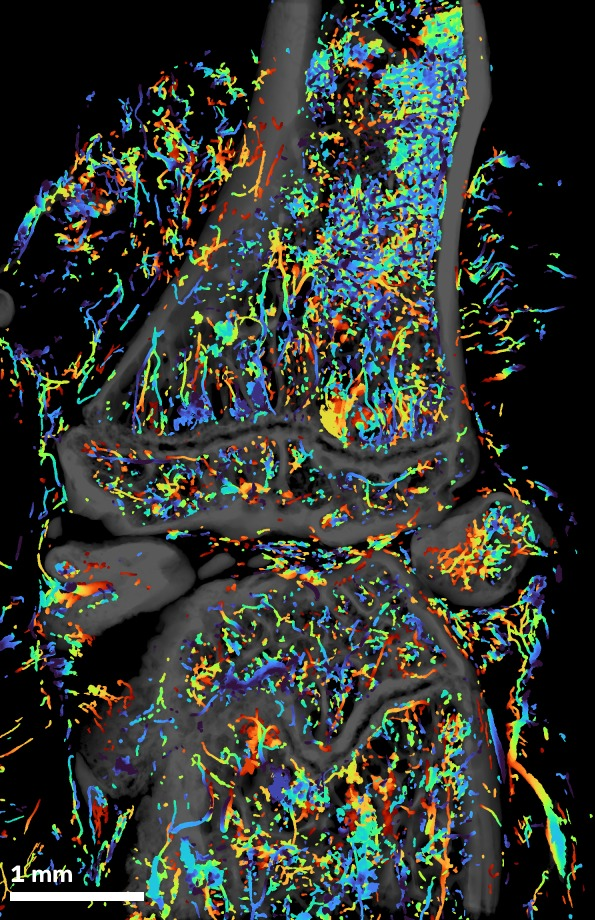
\includegraphics[width=0.62\linewidth]{vessel_network.jpg}
\caption{The vessels of the whole stack seen from above, coloured by depth (blue: first slices, red:
  last slices), over a faint projection of the bone. Marrow vessels of the femur (top) and tibia
  (bottom), and the soft-tissue vessels around the joint.}
\label{fig:network}
\end{figure}
